\documentclass[12pt]{article}

\usepackage{amsmath}

\usepackage{eso-pic}
\usepackage{lipsum}
\usepackage{transparent}
\usepackage{parskip}


\usepackage[utf8]{inputenc}


\usepackage[spanish]{babel} %Paquete de idioma
\usepackage[hidelinks]{hyperref}
\usepackage{graphicx}
\usepackage{float}

\graphicspath{{images/}}

\title{Memoria Práctica 1 \\


\large Sistemas inteligentes
}
\author{
Leopoldo Cadavid Piñeroooooooo
}
\date{Febrero 2022}


%%%%%%%%% ESTO PARA LA MARCA DE AGUA %%%%%%%%%%%%%%%%%%%%%%%%%%%%%%%


\AddToShipoutPicture{ 
    \put(410,380){
        \parbox[b][\paperheight]{\paperwidth}{%
            \vfill
            \
            {
            \transparent{1}
            
\includegraphics[scale=0.5]{logo-ua.png}
            \vfill
            }
        }
    }
}
%%%%%%%%%%%%%%%%%%%%%%%%%%%%%%%%%%%%%%%%%%%%%%%%%%%%%%%%%%




\begin{document}

\maketitle
\newpage
\tableofcontents
\newpage
\section{Introducción}

      En la siguiente memoria se procederá a explicar los diferentes algoritmos de resolución
      empleados para resolver distintos tableros del juego Futoshiki.

      Además, se compararán los resultados de estos en cuanto a su coste temporal,
      Para poder concluir en cual método es el óptimo para el problema propuesto. 
      

\section{Algoritmos impletmentados}
Para cada algoritmo comentaremos las funciones añadidas y la explicación general de su funcionamiento, añadiendo también un apartado comentando fallos o
problemas durante la implementación. Posteriormente, en \ref*{ch:} se comentarán las diferencias temporales 
con los demás algoritmos.

\subsection{Backtracking}
La primera solución implementada para el problema Futoshiki ha sido el 
esquema backtracking. Primero, se comentará la explicación conceptuas de que cómo se ha hecho la implementación
del algoritmo, repasando las funciones y estructuras utilizadas. 
\subsubsection{Funciones y métodos}



\begin{itemize}

    \item \verb|bool bt_futoshiki():| es la función donde se encuentra la estructura
     de resolución backtracking. Devolverá true si se ha llegado a la solución, o false 
     en caso contrario. 

    \item \verb|bool factible():| en esta función se comprueba si el valor 
    seteado en la casilla cumple con las restricciones propias de las reglas de Futoshiki.

    \item \verb|void ejecutarBT():| función por defecto dada en la práctica. Se utilizará
    para obetener los valores iniciales de partida para la solución Backtracking
    y desde esta llamaremos a \verb|bt_futoshiki()|. No se han añadido parámetros a esta ni se han 
    modificado sus propiedades.

    
\end{itemize}

% \begin{figure}[H]
%     \centering
%     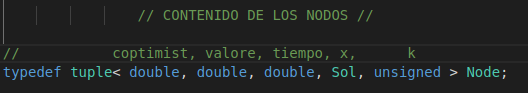
\includegraphics[scale=0.5]{contenido_nodo.png}
%     \caption{Contenido de los nodos}
%     \label{fig:nodo}
% \end{figure}

Entrando más en detalle con el funcionamiento de la función bt\_futoshiki(),
lo que se hace en el código es recorrer el tablero empezando por la superior 
izquierda y para cada posición se comprueban los números de 1 a N. Si el número es factible en esa posición, lo colocamos en la casilla con \verb|setCasilla()|
y llamaremos a la recursividad para seguir comprobando. Si no es factible, comprobamos el siguiente valor posible.

Tras llamar a la recursividad debemos ver si ha devuelto un resultado un resultado verdadero, en cuyo caso se ha encontradola solución y debemos
salir con \textit{true}.

Es importante tener en cuenta que si hemos  comprobado todos los valores posibles y no hay ninguno factible, estamos siguiendo una instanciación errónea y debemos devolver \textit{false}.

En el caso de que en la casilla ya haya un valor prefijado, debemos comprobar aún asi si es factible, pues si
no tendremos que volver hacia atrás. En ningún caso modificamos el valor de la casilla.

También es importante comentar el funcionamiento de \verb|factible()|. En esta función comprobamos si, al poner el valor en la casilla deseada:
 \begin{itemize}
    \item Si el número se repite en la casilla o en la columna.
    \item Si el número cumple las restricciones de \textit{"mayor que"} o \textit{"menor que"} con respecto a la 
        casilla anterior, pues al recorrer el tablero hacia abajo/derecha, comprobar con las casillas a nuestra derecha
        significa que estaríamos comprobando con casillas vacías, lo cual nos llevaría a resultados incorrectos.
 \end{itemize}

\subsubsection{Problemas durante la implementación}

Durante la implementación del algoritmo se dieron algunos problemas, que consiguieron ser solucionados para cumplir con la tarea. Los más destacable:

\begin{itemize}
    \item No se comprobaba si las llamadas recursivas devolvían la solución, con lo cual el algoritmo seguía aplicándose 
    una vez habiendo encontrado la solución.

    \item Al principio no se comprobaba si los números prefijados erán factibles, lo cual daba problemas en el momento 
    en que uno de estos tenía una una restricción binaria con una casilla adyacente. Esto llevaba a resultados incorrectos en 
    tableros como el de 6x6.

    \item No se devolvía falso cuando el algoritmo había descartado todos los números como soluciones factibles de una casilla, lo 
    cual llevaba a una indeterminación en la solución.
\end{itemize}

\subsection{Algoritmo AC3}

\subsubsection{Funciones y métodos}

Para la implementación de este algoritmo, con el fin de seguir la estructura aprendida en clase, se implementaron 
nuevas clases al proyecto, además de añadir nuevos métodos y estructuras.

Primero veamos las clases creadas:

\begin{itemize}
    \item \textbf{Clase nodo:} representa la estructura de datos de un nodo. Se compone de dos enteros que son
    sus coordenadas X e Y.
    \item \textbf{Clase arista:} representa la estructura de datos de una arista. Está compuesta de dos nodos A y B, y
    en el algoritmo consideraremos que la arista tiene dirección de A a B, aunque realmente la arista no tiene una dirección.
    
    \item \textbf{Clase matdominios:} representa el dominio de las casillas del tablero. Se compone de una matriz de 3 dimensiones, 
    donde la primera y segunda serán la fila y columna del tablero. La tercera dimensión representa los números que pueden estar en 
    esa posición, 
\end{itemize}

\textbf{}

\subsubsection{Problemas durante la implementación}
\subsection{Foward Checking}
\begin{figure}[h]
    \centering
    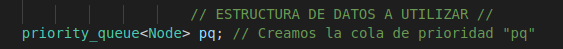
\includegraphics[scale=0.5]{cola_de_prior.png}
    \caption{Implementación de la cola de prioridad}
    \label{fig:colprior}
\end{figure}

\section{}


\end{document}